\section{Expectation Propagation}

\subsection{Introduction}

\begin{remark}{\textbf{(Non-Linear State Space)}}
    We are given the following non-linear space with the following transition and emission probability as we have:
    \begin{equation*}
        \boldsymbol z_{t+1} = f(\boldsymbol z_t, \boldsymbol u_t) + \boldsymbol w_t \qquad \boldsymbol x_t = g(\boldsymbol z_t, \boldsymbol u_t) + \boldsymbol v_t
    \end{equation*}
    where $\boldsymbol w_t$ and $\boldsymbol v_t$ are usually Gaussian, as we can linearlized the non-linear function around $\hat{\boldsymbol z}_t^t$:
    \begin{equation*}
        \boldsymbol z_{t+1} \approx \underbrace{f(\hat{\boldsymbol z}_t^t, \boldsymbol u_t)}_{\tilde{\boldsymbol B}_t\boldsymbol u_t} + \underbrace{\left.\frac{\partial f}{\partial \boldsymbol z_t}\right|_{\hat{\boldsymbol z}^t_t}}_{\tilde{\boldsymbol A}_t}(\boldsymbol z_t - \hat{\boldsymbol z}^t_t) + \boldsymbol w_t \qquad\quad \boldsymbol x_{t} \approx \underbrace{f(\hat{\boldsymbol z}_{t}^{t-1}, \boldsymbol u_t)}_{\tilde{\boldsymbol D}_t\boldsymbol u_t} + \underbrace{\left.\frac{\partial f}{\partial \boldsymbol z_t}\right|_{\hat{\boldsymbol z}^{t-1}_t}}_{\tilde{\boldsymbol C}_t}(\boldsymbol z_t - \hat{\boldsymbol z}^{t-1}_t) + \boldsymbol w_t
    \end{equation*}
    We can run the kalman filter on non-stationary linearized system $( \tilde{\boldsymbol A}_t, \tilde{\boldsymbol B}_t, \tilde{\boldsymbol C}_t,\tilde{\boldsymbol D}_t )$:
    \begin{itemize}
        \item Adaptive approximate non-Gaussian messaage by Gaussian. 
        \item Local linearization depends on central point of distribution, mening that approximation degrads with more stable uncertainty. 
        \item This might work in the system that is close to linear. 
    \end{itemize}
\end{remark}

\begin{remark}{\textbf{(Other Message Approximation)}}
    We have the following message on latent chain:
    \begin{equation*}
    \begin{aligned}
        &P(\boldsymbol z_t | \boldsymbol x_{1:t}) = \frac{1}{Z}P(\boldsymbol x_t | \boldsymbol z_t) \int P(\boldsymbol z_t|\boldsymbol z_{t-1})P(\boldsymbol z_{t-1}|\boldsymbol x_{1:t-1})\dby \boldsymbol z_{t-1} \\
        &\tilde{P}(\boldsymbol z_{t-1} | \boldsymbol x_{1:t-1}) \approx \frac{1}{Z}P(\boldsymbol x_t | \boldsymbol z_t)\int \underbrace{P(\boldsymbol z_t | \boldsymbol z_{t-1})}_{\mathcal{N}(f(\boldsymbol z_{t-1}), \boldsymbol Q)}\underbrace{\tilde{P}(\boldsymbol z_{t-1} | \boldsymbol x_{1:t-1})}_{\mathcal{N}(\hat{\boldsymbol z}_{t-1}, \hat{\boldsymbol V}_{t-1})}\dby \boldsymbol z_{t-1}
    \end{aligned}
    \end{equation*}
    There are several, way to approximate the integration: linearization at the peak (EKF) is only one approach. We can use the Laplace filter use mode and curvature of integrand. Finally, we can use the sigma-point. 
\end{remark}

\begin{remark}{\textbf{(Why not KL?)}}
    We can consider the parametric variational as we have 
    \begin{equation*}
        \operatorname{KL}\brackb{\mathcal{N}(\hat{\boldsymbol z}_t, \hat{\boldsymbol V}) \left\| \int P(\boldsymbol z_t|\boldsymbol z_{t-1})P(\boldsymbol z_{t-1}|\boldsymbol x_{1:t-1})\dby \boldsymbol z_{t-1} \right.}
    \end{equation*}
    This may be hard to find the closed form solution to this KL divergence and we might have to find the value using Monte-Carlo sampling. 
\end{remark}

\subsection{Expectation Propagation}

\begin{proposition}
    Given the $p(\boldsymbol x)$, we let $q$ to be exponential family, where we have:
    \begin{equation*}
        Q(\boldsymbol x) = \frac{\exp\bracka{\boldsymbol T(\boldsymbol x)^T\boldsymbol \theta}}{Z(\boldsymbol \theta)}
    \end{equation*}
    Now, consider the following minimization of: $Q^* = \arg\min_{Q} \operatorname{KL}\Big[ P(\boldsymbol x) \Big\| Q(\boldsymbol x)  \Big]$ is solved when:
    \begin{equation*}
        \brackd{\boldsymbol T(\boldsymbol x)}_{Q^*} = \brackd{\boldsymbol T(\boldsymbol x)}_P
    \end{equation*}
    Or matches the sufficient statistics. 
\end{proposition}
\begin{proof}
    Consider the KL-divergence to be:
    \begin{equation*}
    \begin{aligned}
        \argmin{Q} \operatorname{KL}\Big[ P(\boldsymbol x) \Big\| Q(\boldsymbol x)  \Big] &= \argmin{\boldsymbol \theta}\brackb{ P(\boldsymbol x) \left\| \frac{\exp\bracka{\boldsymbol T(\boldsymbol x)^T\boldsymbol \theta}}{Z(\boldsymbol \theta)} \right.} \\
        &= \argmin{\boldsymbol \theta} - \int P(\boldsymbol x)\log\bracka{\frac{\exp\bracka{\boldsymbol T(\boldsymbol x)^T\boldsymbol \theta}}{Z(\boldsymbol \theta)}} \dby \boldsymbol x \\
        &= \argmin{\boldsymbol \theta} \log(Z(\boldsymbol \theta)) - \int P(\boldsymbol x)\Big[ \boldsymbol T(\boldsymbol x)^T\boldsymbol \theta \Big] \dby \boldsymbol x \\
    \end{aligned}
    \end{equation*}
    The second equality comes from the fact that $\int P(\boldsymbol x)\log P(\boldsymbol x)\dby\boldsymbol x$ is constant. Now, we have the following derivative with respected to $\boldsymbol\theta$:
    \begin{equation*}
    \begin{aligned}
        \frac{\partial}{\partial \boldsymbol \theta}\bracka{\log(Z(\boldsymbol \theta)) - \int P(\boldsymbol x)\Big[ \boldsymbol T(\boldsymbol x)^T\boldsymbol \theta \Big] \dby \boldsymbol x } &= \frac{1}{Z(\boldsymbol \theta)}\frac{\partial}{\partial \boldsymbol \theta} \int \exp(\boldsymbol T(\boldsymbol x)^T\boldsymbol \theta)\dby \boldsymbol x - \int p(\boldsymbol x)T(\boldsymbol x)\dby \boldsymbol x \\
        &= \frac{1}{Z(\boldsymbol \theta)}\int \exp(\boldsymbol T(\boldsymbol x)^T\boldsymbol \theta) T(\boldsymbol x)\dby \boldsymbol x - \brackd{T(\boldsymbol x)}_{P} \\
        &= \brackd{T(\boldsymbol x)}_P - \brackd{T(\boldsymbol x)}_Q
    \end{aligned}
    \end{equation*}
    Setting this to zero as we have the solution.  
\end{proof}

\begin{remark}{\textbf{(KL-Divergence Solution)}}
    It is better for use to perform the following KL minimization:
    \begin{equation*}
        \operatorname{KL}\brackb{\left. \int P(\boldsymbol z_t|\boldsymbol z_{t-1})P(\boldsymbol z_{t-1}|\boldsymbol x_{1:t-1})\dby \boldsymbol z_{t-1} \right\|  \mathcal{N}(\hat{\boldsymbol z}_t, \hat{\boldsymbol V}) }
    \end{equation*}
    As we can consider the expected sufficient statistics of the real distribution, instead of finding the exact version of it. However, to calculate the expected sufficient statistics $\brackd{\boldsymbol T(\boldsymbol x)}_P$, which may be analytically tractable, however for the high-dimensional integral (we can use various algorithms to calculate the expectation).
\end{remark}

\begin{remark}{\textbf{(Another Problem of KL-Divergence)}}
    Let's consider the KL-divergence of the factored model, as we have:
    \begin{equation*}
    \begin{aligned}
        \argmin{q_i} \operatorname{KL}\brackb{P(\mathcal{Z} | \mathcal{X}) \left\| \prod_j q_j(\mathcal{Z}_j | \mathcal{X}) \right.} &= \argmin{q_i} -\int P(\mathcal{Z} | \mathcal{X})\log \prod_j q_j(\mathcal{Z}_j | \mathcal{X})\dby\mathcal{Z} \\
        &= \argmin{q_i} - \sum_j \int P(\mathcal{Z}|\mathcal{X})\log q_j(\mathcal{Z}_j|\mathcal{X})\dby\mathcal{Z} \\
        &=  \argmin{q_i} - \int P(\mathcal{Z}_i|\mathcal{X})\log q_i(\mathcal{Z}_i|\mathcal{X})\dby\mathcal{Z}_i \\
        &= P(\mathcal{Z}_i | \mathcal{X})
    \end{aligned}
    \end{equation*}
    We will have to know the marginal, which is intractable. 
\end{remark}

\begin{remark}{\textbf{(EP Motivation)}}
    The posterior distribution in a graphical model is a product of factors:
    \begin{equation*}
        P(\mathcal{Z}|\mathcal{X}) = \frac{P(\mathcal{Z}, \mathcal{X})}{P(\mathcal{X})} = \frac{1}{Z}\prod_i P(\mathcal{Z}_i | \operatorname{Pa}(\mathcal{Z}_i)) \propto \prod_i f_i(\mathcal{Z}_i)
    \end{equation*}
    where $Z_i$ isn't necessary disjoint and we call $f_i$ sites, we consider the same factorization, but with approximate site as we have:
    \begin{equation*}
        \min_{\tilde{f}_i}\operatorname{KL}\brackb{ f_i(\mathcal{Z}_i) \prod_{j\ne i}\tilde{f}_j(\mathcal{Z}_j) \left\| \tilde{f}_i(\mathcal{Z}_i) \prod_{j\ne i}\tilde{f}_j(\mathcal{Z}_j) \right.} \iff \min_{f} \operatorname{KL}\brackb{ f_i(\mathcal{Z}_i) q_{\neg i}(\mathcal{Z}) \Big\| f(\mathcal{Z}_i)q_{\neg i}(\mathcal{Z}) }
    \end{equation*}
    where we have $q_{\neg i}(\mathcal{Z}) = \prod_{j\ne i}\tilde{f}_j(\mathcal{Z}_j)$. This leads to $2$ ideas about expectation propagation as:
    \begin{itemize}
        \item \emph{Expectation}: Approximation of factors, where we perform a projection to exponential family, thus requiring a sufficient statistics. 
        \item \emph{Propagation}: Local divergence minimization leads to message passing approach (hence the number of propagation).
    \end{itemize}
\end{remark}

\begin{proposition}{\textbf{(Simplier Update)}}
    If we consider the context factor, as $q_{\neg i}(\mathcal{Z}) = \textcolor{red}{q_{\neg i}(\mathcal{Z}_i)}q_{\neg i}(\mathcal{Z}_{\neg i} | \mathcal{Z}_i) $ and we have $\mathcal{Z}_{\neg i} = \mathcal{Z}\backslash \mathcal{Z}_{i}$ we can show that:
    \begin{equation*}
        \min_f \operatorname{KL}\brackb{ f_i(\mathcal{Z}_i)\textcolor{blue}{q_{\neg i}(\mathcal{Z})} \Big\| f(\mathcal{Z}_i)\textcolor{blue}{q_{\neg i}(\mathcal{Z})} } \equiv \min_f \operatorname{KL}\brackb{ f_i(\mathcal{Z}_i)\textcolor{red}{q_{\neg i}(\mathcal{Z}_i)} \Big\| f(\mathcal{Z}_i)\textcolor{red}{q_{\neg i}(\mathcal{Z}_i)} }
    \end{equation*}
    Please see that the differences between those $2$ between \textcolor{red}{red} and \textcolor{blue}{blue}. We call $q_{\neg i}(\mathcal{Z}_i)$
\end{proposition}
\begin{proof}
    Consider the following equalities:
    \begin{equation*}
    \begin{aligned}
        \min_f \operatorname{KL}\Big[ f_i(\mathcal{Z}_i)\textcolor{blue}{q_{\neg i}(\mathcal{Z})} &\Big\| f(\mathcal{Z}_i)\textcolor{blue}{q_{\neg i}(\mathcal{Z})} \Big] = \max_f \int f_i(\mathcal{Z}_i)q_{\neg i}(\mathcal{Z})\log\Big[ f(\mathcal{Z}_i)q_{\neg i}(\mathcal{Z}) \Big]\dby\mathcal{Z} \\
        &= \max_f \int f_i(\mathcal{Z}_i) q_{\neg i}(\mathcal{Z}_i)q_{\neg i}(\mathcal{Z}_{\neg i} | \mathcal{Z}_i) \log\Big[ f(\mathcal{Z}_i) q_{\neg i}(\mathcal{Z}_i)q_{\neg i}(\mathcal{Z}_{\neg i} | \mathcal{Z}_i) \Big]\dby\mathcal{Z}_i\dby\mathcal{Z}_{\neg i} \\
        &= \max_f \int f_i(\mathcal{Z}_i) q_{\neg i}(\mathcal{Z}_i)q_{\neg i}(\mathcal{Z}_{\neg i} | \mathcal{Z}_i) \Big[ \log f(\mathcal{Z}_i) q_{\neg i}(\mathcal{Z}_i)\Big]\dby\mathcal{Z}_i\dby\mathcal{Z}_{\neg i} \\
        &= \max_f \int f_i(\mathcal{Z}_i) q_{\neg i}(\mathcal{Z}_i) \Big[ \log f(\mathcal{Z}_i) q_{\neg i}(\mathcal{Z}_i)\Big]\dby\mathcal{Z}_i \int q_{\neg i}(\mathcal{Z}_{\neg i} | \mathcal{Z}_i) \dby\mathcal{Z}_{\neg i} \\
        &= \min_f \operatorname{KL}\brackb{ f_i(\mathcal{Z}_i){q_{\neg i}(\mathcal{Z}_i)} \Big\| f(\mathcal{Z}_i){q_{\neg i}(\mathcal{Z}_i)} }
    \end{aligned}
    \end{equation*}
    And so the equality is proven.
\end{proof}

\begin{definition}{\textbf{(Expectation Propagation)}}
    We consider the following algorithms for expectation propagation, pseudocode:
    \begin{algorithm}[H]
        \caption{Expectation Propagation Algorithm}
        \begin{algorithmic}[1]
            \State \textbf{Input}: $f_1(\mathcal{Z}_1),\dots,f_N(\mathcal{Z}_N)$
            \State \textbf{Initilize}: $\tilde{f}_i(\mathcal{Z}_i) = 1$ for $i\in[n]$ and we have $q(\mathcal{Z}) \propto \prod_i\tilde{f}_i(\mathcal{Z}_i)$
            \While{convergence}
            \For {$i=1,2,\cdots, N$}
                \State \emph{Delete}: We do the update to get the cavity 
                \begin{equation*}
                    q_{\neg i}(\mathcal{Z}) \leftarrow \frac{q(\mathcal{Z})}{\tilde{f}_i(\mathcal{Z}_i)} = \prod_{j\ne i}\tilde{f}_j(\mathcal{Z}_j)
                \end{equation*}
                \State \emph{Project}: Performing KL-divergence minimization
                \begin{equation*}
                    \tilde{f}^\text{new}_i(\mathcal{Z}) \leftarrow \argmin{f} \operatorname{KL}\brackb{f_i(\mathcal{Z}_i)q_{\neg i}(\mathcal{Z}_i) \Big\| f(\mathcal{Z}_i)q_{\neg i}(\mathcal{Z}_i) }
                \end{equation*}
                \State \emph{Include}: $q(\mathcal{Z}) \leftarrow \tilde{f}^\text{new}_i(\mathcal{Z}_i)q_{\neg i}(\mathcal{Z})$
            \EndFor
            \EndWhile
        \end{algorithmic} 
    \end{algorithm}
\end{definition}

\begin{remark}{\textbf{(Calculate the Cavity Distribution)}}
    The cavity distribution can be broken down into product of terms for each neighboring cliques:
    \begin{equation*}
        q_{\neg i}(\mathcal{Z}_i) = \prod_{j\in\operatorname{ne}(i)} M_{j\rightarrow i}(\mathcal{Z}_i\cap\mathcal{Z}_j)
    \end{equation*}
    The i-th site has been approximated as the message can be passed onto neighboring cliques by normalizing the shared variable. This is belief propagation. Furthermore, the message updates can be scheduled in any order. However, there is no guarantee of convergence. 
\end{remark}

\begin{remark}{\textbf{(Normalizer)}}
    As long as approximating class is tractable, normalizer can be computed as needed. Consider the approximation class to be:
    \begin{equation*}
        \tilde{f}_i(\mathcal{Z}_i) \propto \exp\Big( \boldsymbol T(\mathcal{Z})^T\boldsymbol \theta_i - \Phi(\boldsymbol \theta_i) \Big)
    \end{equation*}
    This is the same as setting every entries $\boldsymbol \theta_i$ to $0$ except for the one that is in $\mathcal{Z}_i$ (while finding the sufficient statistics for all latents). This will give us the following probability:
    \begin{equation*}
        q(\mathcal{Z}) \propto \prod_i\tilde{f}_i \propto \exp\bracka{\boldsymbol T(\mathcal{Z})^T\sum_i\boldsymbol \theta_i - \sum_i\Phi(\boldsymbol \theta_i)}
    \end{equation*}
    We can re-normalizied it as we have $q(\mathcal{Z}) = \exp\bracka{\boldsymbol T(\mathcal{Z})^T\sum_i\boldsymbol \theta_i - \Phi\bracka{\sum_i\boldsymbol \theta_i}}$
\end{remark}

\begin{remark}{\textbf{(Computing Likelihood)}}
    Consider the unnormalized exponential family, where we have the approximating site to be:
    \begin{equation*}
        \tilde{f}_i = \tilde{C}_i\exp\Big( \boldsymbol T(\mathcal{Z})^T\boldsymbol \theta_i \Big)
    \end{equation*}
    We consider the following values 
    \begin{itemize}
        \item $\boldsymbol \theta = \sum_i\boldsymbol \theta_i$, which is the natural parameter of $q(\mathcal{Z})$
        \item $\boldsymbol \theta_{\neg i} = \sum_{j\ne i}\boldsymbol \theta_i$ as the natural parameter of $q_{\neg i}(\mathcal{Z})$
        \item Exponential family (tractable) log-normalizer $\boldsymbol \Phi(\boldsymbol \theta)$ of $P(\mathcal{Z})$ to be:
        \begin{equation*}
            \boldsymbol \Phi(\boldsymbol \theta) = \log \int \exp(\boldsymbol T(\mathcal{Z})^T\boldsymbol \theta) \dby \mathcal{Z}
        \end{equation*}
    \end{itemize}
    Now, we are interested to find the actual approximation of the normalizer i.e:
    \begin{equation*}
        \log \int \prod^N_{i=1}f_i(\mathcal{Z}_i)
    \end{equation*}
    To do this, we minimize the unnormalized KL divergence (where we also care about the normalizer, see the additional term):
    \begin{equation*}
        \operatorname{KL}_\text{un}[p\| q] = \int p(\boldsymbol x)\log \frac{p(\boldsymbol x)}{q(\boldsymbol x)}\dby \boldsymbol x + \int \Big( q(\boldsymbol x) - p(\boldsymbol x) \Big)\dby \boldsymbol x
    \end{equation*}
\end{remark}

\begin{proposition}{\textbf{(Log Likelihood Approximation)}}
    The approximation of the log-likelihood is given as:
    \begin{equation*}
        \log \int \prod^N_{i=1}f_i(\mathcal{Z}_i) \approx \log \int \prod^N_{i=1}\tilde{f}_i(\mathcal{Z}_i) = (1- N)\Phi(\boldsymbol \theta) + \sum_{i=1}^N \Phi_i(\boldsymbol \theta_{\neg i})
    \end{equation*}
    where $\boldsymbol \Phi_i$ is the log-normalizer of the distribution $\hat{P}_i(\mathcal{Z}) \propto f(\mathcal{Z})\exp(\boldsymbol T(\mathcal{Z})^T\boldsymbol \theta)$
\end{proposition}
\begin{proof}
    To follows the unnormalized KL divergence, the first terms simply follows the expected sufficient statistics match. In this case, we have (thinking of it as having KL-divergence equal to zero):
    \begin{equation*}
    \begin{aligned}
        \min_{\tilde{C}_i}&\operatorname{KL}_\text{min}\brackb{ \tilde{C}_i\exp\Big( \boldsymbol T(\mathcal{Z})^T\boldsymbol \theta_i \Big) \prod_{\neg i} \tilde{C}_j\exp\Big( \boldsymbol T(\mathcal{Z})^T\boldsymbol \theta_j \Big) \left\| f_i(\mathcal{Z}_i)\prod_{\neg i} \tilde{C}_j\exp\Big( \boldsymbol T(\mathcal{Z})^T\boldsymbol \theta_j \Big) \right.} \\
        \iff& \int \tilde{C}_i\exp\Big( \boldsymbol T(\mathcal{Z})^T\boldsymbol \theta_i \Big) \prod_{\neg i} \tilde{C}_j\exp\Big( \boldsymbol T(\mathcal{Z})^T\boldsymbol \theta_j \Big) \dby \mathcal{Z} = \int f_i(\mathcal{Z}_i)\prod_{\neg i} \tilde{C}_j\exp\Big( \boldsymbol T(\mathcal{Z})^T\boldsymbol \theta_j \Big) \dby \mathcal{Z} \\
        \iff& \int \tilde{C}_i \prod_{i}\exp\Big( \boldsymbol T(\mathcal{Z})^T\boldsymbol \theta_j \Big) \dby \mathcal{Z} = \int f_i(\mathcal{Z}_i)\prod_{\neg i} \exp\Big( \boldsymbol T(\mathcal{Z})^T\boldsymbol \theta_j \Big) \dby \mathcal{Z} \\
        \iff& \tilde{C}_i \exp(\boldsymbol \Phi(\boldsymbol \theta)) = \exp(\boldsymbol \Phi_i(\boldsymbol \theta_{\neg i})) \\
        \iff& \tilde{C}_i = \exp\Big(\boldsymbol \Phi_i(\boldsymbol \theta_{\neg i}) - \boldsymbol \Phi(\boldsymbol \theta) \Big)
    \end{aligned}
    \end{equation*}
    and so, we have the following log-likelihood to be:
    \begin{equation*}
    \begin{aligned}
        \log \int \prod^N_{i=1}\tilde{f}_i(\mathcal{Z}_i)\dby\mathcal{Z} &= \log \int \prod^N_{i=1}\tilde{C}_i\exp\Big( \boldsymbol T(\mathcal{Z})^T\boldsymbol \theta_i \Big)\dby\mathcal{Z} \\
        &= \log \prod^N_{i=1}\tilde{C}_i \int \exp\bracka{\boldsymbol T(\mathcal{Z})^T\brackb{\sum^N_{i=1}\boldsymbol \theta_i }}\dby\mathcal{Z} \\
        &=\boldsymbol \Phi(\boldsymbol \theta) + \sum^N_{i=1} \log \tilde{C}_i  = (1- N)\Phi(\boldsymbol \theta) + \sum_{i=1}^N \Phi_i(\boldsymbol \theta_{\neg i})
    \end{aligned}
    \end{equation*}
\end{proof}

\subsection{Examples}

\begin{remark}{\textbf{(Example: Non-Linear State Space Model)}}
    Consider the graphical model: 
    \begin{figure}[H]
        \centering
        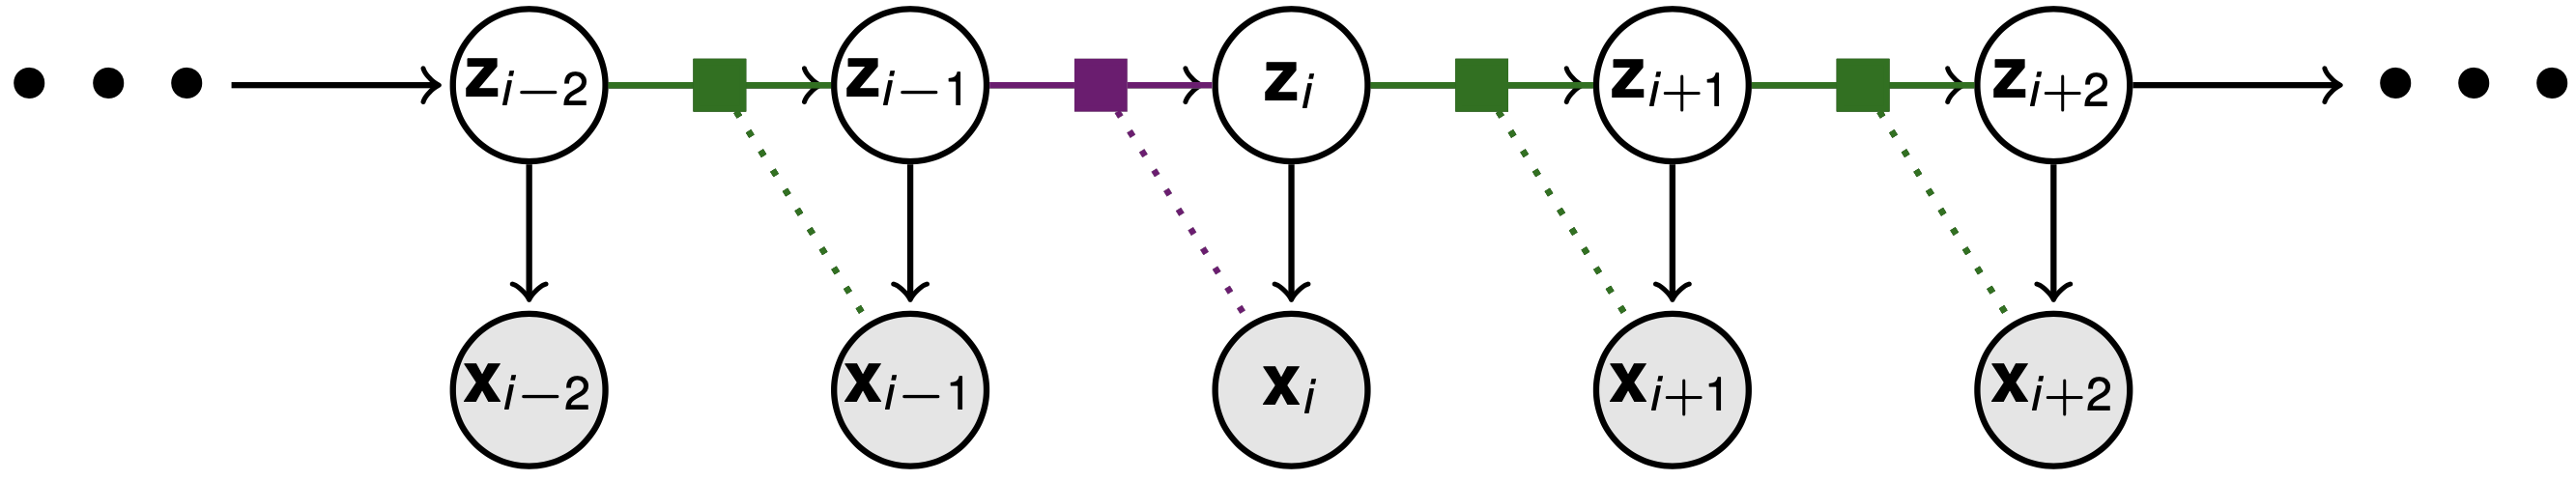
\includegraphics[width=10cm]{img/img14.png}
    \end{figure}  
    where we have the following factors:
    \begin{equation*}
    \begin{aligned}
        &P(\boldsymbol z_i | \boldsymbol z_{i-1}) = \phi_i(\boldsymbol z_i, \boldsymbol z_{i-1}) = \exp\bracka{-\frac{\norm{\boldsymbol z_i - h_s(\boldsymbol z_i)}^2}{2\sigma^2}} \\
        &P(\boldsymbol x_i | \boldsymbol z_i) = \psi_i(\boldsymbol z_i) = \exp\bracka{-\frac{\norm{\boldsymbol x_i - h_o(\boldsymbol z_i)}^2}{2\sigma^2}}
    \end{aligned}
    \end{equation*}
    We can see that $f_i(\boldsymbol z_i, \boldsymbol z_{i-1}) = \phi_i(\boldsymbol z_i, \boldsymbol z_{i-1})\psi_i(\boldsymbol z_i)$ as there are non-linear, the inference isn't generally tractable. For the EP, we will consider the approximate $\tilde{f}(\boldsymbol z_i, \boldsymbol z_{i-1})$ to be Gaussian as we have. Consider the cavity distribution to be:
    \begin{equation*}
    \begin{aligned}
        q_{\neg i}(\boldsymbol z_i, \boldsymbol z_{i-1}) &= \int_{\boldsymbol z_1,\dots,\boldsymbol z_{i-2}, \boldsymbol z_{i+1}, \dots, \boldsymbol z_n} \prod_{i'\ne i}\tilde{f}_{i'}(\boldsymbol z_{i'}, \boldsymbol z_{i'-1}) \\
        &= \underbrace{\int_{\boldsymbol z_1,\dots,\boldsymbol z_{i-2}}\prod_{i'<i} \tilde{f}_{i'}(\boldsymbol z_{i'}, \boldsymbol z_{i'-1})}_{\alpha_{i-1}(\boldsymbol z_{i-1})}\underbrace{\int_{\boldsymbol z_{i+1},\dots,\boldsymbol z_n}\prod_{i'>i} \tilde{f}_{i'}(\boldsymbol z_{i'}, \boldsymbol z_{i'-1})}_{\beta_i(\boldsymbol z_i)}
    \end{aligned}
    \end{equation*}
    Please note that $\alpha, \beta$ is being Gaussian (by default), and so we have the following update rule:
    \begin{equation*}
        \tilde{f}_i(\boldsymbol z_i, \boldsymbol z_{i-1}) = \argmin{f\in\mathcal{N}} \operatorname{KL}\brackb{ \phi_i(\boldsymbol z_i, \boldsymbol z_{i-1})\psi_i(\boldsymbol z_i)\alpha_{i-1}(\boldsymbol z_{i-1})\beta_i(\boldsymbol z_i) \Big\| f(\boldsymbol z_i, \boldsymbol z_{t-1}) \alpha_{i-1}(\boldsymbol z_{i-1})\beta_i(\boldsymbol z_i) }
    \end{equation*}
    We can consider the following optimization instead as we have:
    \begin{equation*}
    \begin{aligned}
        \tilde{P}(\boldsymbol z_{i-1}, \boldsymbol z_i) &= \argmin{P\in\mathcal{N}}\operatorname{KL}\brackb{ \hat{P}(\boldsymbol z_{i-1}, \boldsymbol z_i) \Big\| P(\boldsymbol z_{i-1}, \boldsymbol z_i) } \\
        \implies&  \tilde{f}_i(\boldsymbol z_i, \boldsymbol z_{i-1}) = \frac{\tilde{P}(\boldsymbol z_{i-1}, \boldsymbol z_i)}{\alpha_{i-1}(\boldsymbol z_{i-1})\beta_i(\boldsymbol z_i) }
    \end{aligned}
    \end{equation*}
    Now, we consider each values $\alpha_i(\boldsymbol z_i)$ and $\beta_{i-1}(\boldsymbol z_{t-1})$ as the propagation step:
    \begin{equation*}
    \begin{aligned}
        &\alpha_i(\boldsymbol z_i) = \int_{\boldsymbol z_1,\dots,\boldsymbol z_{i-1}} \prod_{i' < i+1}\tilde{f}_{i'}(\boldsymbol z_{i'}, \boldsymbol z_{i'-1}) = \int_{\boldsymbol z_i}\alpha_{i-1}(\boldsymbol z_{i-1})\tilde{f}_i(\boldsymbol z_i, \boldsymbol z_{i-1}) = \frac{1}{\beta_i(\boldsymbol z_i)} \int_{\boldsymbol z_{i-1}} \tilde{P}(\boldsymbol z_{i-1}, \boldsymbol z_i)\dby \boldsymbol z_{i-1} \\
        &\beta_{i-1}(\boldsymbol z_{i-1}) = \int_{\boldsymbol z_{i},\dots,\boldsymbol z_{n}}\prod_{i' < i+1}\tilde{f}_{i'}(\boldsymbol z_{i'}, \boldsymbol z_{i'-1}) = \int_{\boldsymbol z_i}\beta_i(\boldsymbol z_i)\tilde{f}_i(\boldsymbol z_i, \boldsymbol z_{i-1}) = \frac{1}{\alpha_{i-1}(\boldsymbol z_{i-1})} \int_{\boldsymbol z_i} \tilde{P}(\boldsymbol z_{i-1}, \boldsymbol z_i)\dby \boldsymbol z_i
    \end{aligned}
    \end{equation*}
    The last equality comes from the another definition of $\tilde{f}_i(\boldsymbol z_{i-1}, \boldsymbol z_i)$. The update of both $\alpha_i$ and $\beta_i$ are marginalization of $\tilde{P}(\boldsymbol z_{i-1}, \boldsymbol z_i)$, which is also a Gaussian.
\end{remark}


\begin{remark}{\textbf{(EP For GP Classification)}}
    We can write the GP joint on $g_i$ and $y_i$ as a factor graph:
    \begin{figure}[H]
        \centering
        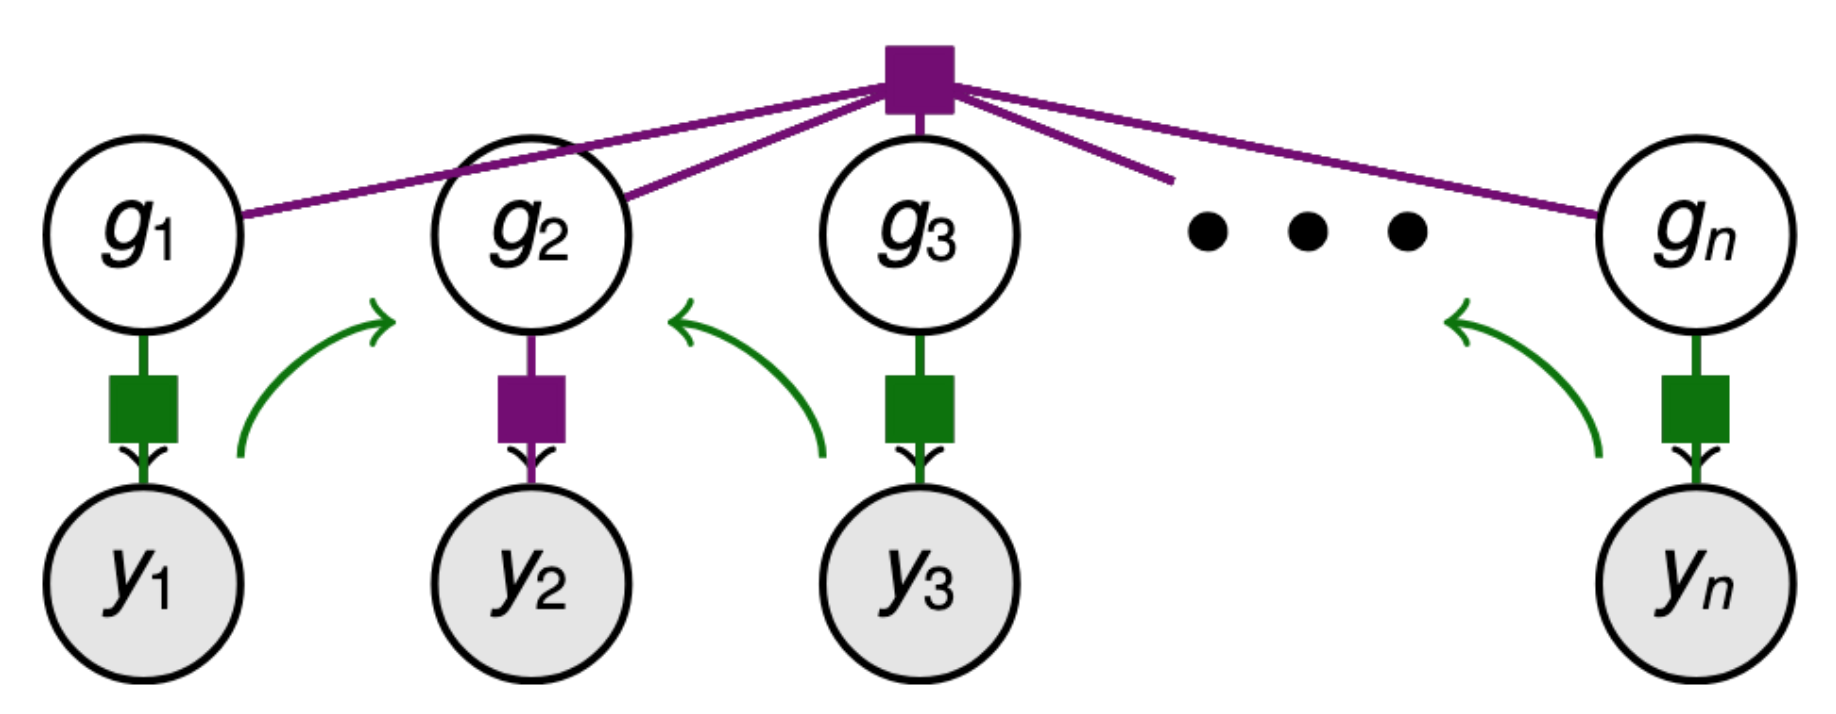
\includegraphics[width=8cm]{img/img15.png}
    \end{figure}  
    Consider the following factorization:
    \begin{equation*}
        P(g_1,\dots,g_n,y_1,\dots,y_n) = \underbrace{\mathcal{N}(g_1,\dots,g_n|0, K)}_{f_0(\mathcal{G})} \prod_i \underbrace{P(y_i|g_i)}_{f_i(g_i)}
    \end{equation*}
    Some factorization applied to non-Gaussian $P(y_i = 1 | g_i) = 1/(1+\exp(-g_i))$. EP approximate non-Gaussian $f_i(g_i)$ by Gaussian to be $\tilde{f}_i(g_i) = \mathcal{N}(\tilde{\mu}_i, \tilde{\psi}_i^2)$. Given $q_{\neg i}(g_i)$ can be concluded by GP marginalization:
    \begin{equation*}
        q_{\neg i}(g_i) = \mathcal{N}\Big( \boldsymbol \Sigma_{i, \neg i}\boldsymbol \Sigma^{-1}_{\neg i, \neg i} \tilde{\boldsymbol \mu}_{\neg i}, \ K_{i,i} - \boldsymbol \Sigma_{i, \neg i} \boldsymbol \Sigma^{-1}_{\neg i, \neg i}\boldsymbol \Sigma_{\neg i, i} \Big)
    \end{equation*}
    We will consider $\boldsymbol \Sigma = \boldsymbol K + \operatorname{diag}(\tilde{\psi}^2_1,\dots,\tilde{\psi}^2_n)$. The update on the Gaussian is based on sufficient statistics matching where $P(g) = f_i(g)q_\neg(g)$, as now we have the follow:
    \begin{equation*}
        \tilde{f}_\text{new}(g_i) = \left.\mathcal{N}\bigg( \underbrace{\int q_{\neg i}(g)f_i(g)g\dby g}_{\tilde{\mu}^\text{new}_i}, \ \int q_{\neg i}(g)f_i(g)g^2\dby g -  (\tilde{\mu}^\text{new}_i)^2 \bigg)\right/q_{\neg i}(g_i)
    \end{equation*}
    Once approximation site potential have stabilize, we use them to make a prediction from $\boldsymbol x'$. There are some observations that we made:
    \begin{itemize}
        \item Introduce the prediction point will changes $\boldsymbol K$, but it will not affect the marginal. 
        \item The unobserved output factor proved no information about $g'$ (the output of $\boldsymbol x'$) and so we don't have to approximate potential $\tilde{f}_i$
        \item And so, we have the following prediction:
        \begin{equation*}
            P(y' | \boldsymbol x', \mathcal{D}) = \int P(y' | \boldsymbol g')\mathcal{N}\bracka{ \boldsymbol g' \Big|  \boldsymbol K_{x'X}(\boldsymbol K_{XX} + \tilde{\boldsymbol \Psi})^{-1} \tilde{\boldsymbol \mu}, \ \boldsymbol K_{x'x'}(\boldsymbol K_{XX} + \tilde{\boldsymbol \Psi})^{-1}\boldsymbol K_{Xx'} } \dby \boldsymbol g'
        \end{equation*}
        where $\tilde{\boldsymbol \Psi} = \operatorname{diag}(\tilde{\psi}^2_1,\dots,\tilde{\psi}^2_n)$. 
    \end{itemize}
\end{remark}

\subsection{Learning with EP}

\begin{remark}{\textbf{(Learning and EP)}}
    EP can yields the approximate inference posterior. To learn the hyperparameter as we can use:
    \begin{itemize}
        \item Approximate Bayesian inference (like VB): Maybe need to construct a coherent normalizable exponential familty on both latent and parameter. 
        \item Approximate EM: As we can maximize $\brackd{\log P(\mathcal{X}, \mathcal{Z})}_{q_\text{EP}(\mathcal{Z})}$. It is practical but not coherent cost function so no guarantee of convergence even if EP itself converges. 
        \item Direct maximization of EP log-likelihood estimate:
        \begin{itemize}
            \item Consistent although convergence guarantee still difficult. 
            \item Seem hard to differentiate, but it is simpler than what it looks like.
        \end{itemize}
    \end{itemize}
\end{remark}

\begin{proposition}
    We can show that the EP of the moment matching as we now have:
    \begin{equation*}
        \nabla_\eta \tilde{l} = \sum^N_{i=1}\brackd{\nabla_\eta \log f_i(\mathcal{Z}_i)}_{\hat{P}_i}
    \end{equation*}
    where $\eta$ is the model hyperparameter. It can be computed provided that EP converges.
\end{proposition}
\begin{proof}
    Let's consider the derivative of $\log \tilde{C}_i$ as we have:
    \begin{equation*}
    \begin{aligned}
        \nabla_\eta \log \tilde{C}_i &= \nabla_\eta \boldsymbol \Phi_i(\boldsymbol \theta_{\neg i}) - \nabla_\eta \boldsymbol \Phi(\boldsymbol \theta) = \nabla_\eta \boldsymbol \Phi_i(\boldsymbol \theta_{\neg i}) - \boldsymbol\mu^T\nabla_\eta\boldsymbol\theta \\
    \end{aligned}
    \end{equation*}
    Please recall the gradient of the log normalizer in the first equality i.e $\boldsymbol\mu = \brackd{\boldsymbol T(\mathcal{Z})}_{q(\mathcal{Z})}$. We will have to consider $\nabla_\eta \boldsymbol \Phi_i(\boldsymbol \theta_{\neg i})$ as we have (it depends on $\eta$ via $f_i$ and $\boldsymbol\theta_{\neg i}$):
    \begin{equation*}
    \begin{aligned}
        \nabla_\eta &\boldsymbol \Phi_i(\boldsymbol \theta_{\neg i}) = \frac{1}{\exp(\boldsymbol \Phi_i(\boldsymbol \theta_{\neg i}))}\brackb{ \int \exp\bracka{\boldsymbol T(\mathcal{Z})^T\boldsymbol \theta_{\neg i}}\nabla_\eta f_i(\mathcal{Z}_i) \dby\mathcal{Z} + \int f_i(\mathcal{Z}_i)\nabla_\eta \exp\brackb{\boldsymbol T(\mathcal{Z})^T\boldsymbol \theta_{\neg i}} } \\
        &= \frac{1}{\exp(\boldsymbol \Phi_i(\boldsymbol \theta_{\neg i}))}\int \exp\bracka{\boldsymbol T(\mathcal{Z})^T\boldsymbol \theta_{\neg i}}\nabla_\eta f_i(\mathcal{Z}_i) \dby\mathcal{Z} +  \int \frac{f_i(\mathcal{Z}_i) \exp\bracka{\boldsymbol T(\mathcal{Z})^T\boldsymbol \theta_{\neg i}}}{\exp(\boldsymbol \Phi_i(\boldsymbol \theta_{\neg i}))} \boldsymbol T(\mathcal{Z})^T\nabla_\eta \boldsymbol \theta_{\neg i} \dby\mathcal{Z} \\
        &= \int \frac{f_i(\mathcal{Z}_i)\exp\bracka{\boldsymbol T(\mathcal{Z})^T\boldsymbol \theta_{\neg i}}}{\exp(\boldsymbol \Phi_i(\boldsymbol \theta_{\neg i}))}\nabla_\eta \log f_i(\mathcal{Z}_i) \dby\mathcal{Z} +  \int \frac{f_i(\mathcal{Z}_i) \exp\bracka{\boldsymbol T(\mathcal{Z})^T\boldsymbol \theta_{\neg i}}}{\exp(\boldsymbol \Phi_i(\boldsymbol \theta_{\neg i}))} \boldsymbol T(\mathcal{Z})^T\nabla_\eta \boldsymbol \theta_{\neg i} \dby\mathcal{Z} \\
        &= \brackd{\nabla_\eta \log f_i(\mathcal{Z}_i)}_{\hat{P}_i} + \brackd{\boldsymbol T(\mathcal{Z})}^T_{\hat{P}_i}\nabla_\eta \boldsymbol \theta_{\neg i} \\
        &= \brackd{\nabla_\eta \log f_i(\mathcal{Z}_i)}_{\hat{P}_i} + \boldsymbol \mu^T \nabla_\eta \boldsymbol \theta_{\neg i} \\
    \end{aligned}
    \end{equation*}
    Consider the derivative with respected to the hyperparameter as we have:
    \begin{equation*}
    \begin{aligned}
        \nabla_\eta \tilde{l} &= \nabla_\eta \boldsymbol \Phi(\boldsymbol \theta) + \sum^N_{i=1}\nabla_\eta \log \tilde{C}_i \\
        &= \boldsymbol\mu^T\nabla_\eta \boldsymbol \theta + \sum^N_{i=1}\Big( \brackd{\nabla_\eta \log f_i(\mathcal{Z}_i)}_{\hat{P}_i} + \boldsymbol \mu^T\nabla_\eta \boldsymbol \theta_{\neg i} - \boldsymbol\mu^T\nabla_\eta\boldsymbol\theta \Big)  \\
        &= \boldsymbol\mu^T\nabla_\eta\bracka{ \sum^N_{i=1}\boldsymbol \theta_i + \sum^N_{i=1}(\boldsymbol \theta_{\neg i} - \boldsymbol \theta)} + \sum^N_{i=1}\Big( \brackd{\nabla_\eta \log f_i(\mathcal{Z}_i)}_{\hat{P}_i}\Big)  \\
        &= \boldsymbol\mu^T\nabla_\eta\bracka{\sum^N_{i=1}(\boldsymbol \theta - \boldsymbol \theta)} + \sum^N_{i=1}\brackd{\nabla_\eta \log f_i(\mathcal{Z}_i)}_{\hat{P}_i}  \\
        &=\sum^N_{i=1}\brackd{\nabla_\eta \log f_i(\mathcal{Z}_i)}_{\hat{P}_i}  \\
    \end{aligned}
    \end{equation*}
    Thus complete the proof
\end{proof}

\begin{definition}{\textbf{(Alpha Divergence)}}
    This is a generalization of the KL-divergence to be:
    \begin{equation*}
        D_\alpha[p \| q] = \frac{1}{\alpha(1-\alpha)} \int \alpha p(\boldsymbol x) + (1-\alpha)q(\boldsymbol x) - p(\boldsymbol x)^\alpha q(\boldsymbol x)^{1-\alpha}\dby \boldsymbol x
    \end{equation*} 
\end{definition}

\begin{remark}
    We have the following values for $\alpha$ as we have:
    \begin{itemize}
        \item For $\alpha = -1$:
        \begin{equation*}
            D_{-1}[p\| q] = \frac{1}{2}\int \frac{(p(\boldsymbol x)-q(\boldsymbol x))^2}{p(\boldsymbol x)}\dby \boldsymbol x
        \end{equation*}
        \item For $\alpha = 1/2$:
        \begin{equation*}
            D_{1/2}[p\|q] = 2 \int\bracka{p(\boldsymbol x)^{1/2} - q(\boldsymbol x)^{1/2}}^2\dby \boldsymbol x
        \end{equation*}
        \item For $\alpha = 2$:
        \begin{equation*}
            D_2[p\|q] = \frac{1}{2}\int \frac{(p(\boldsymbol x)-q(\boldsymbol x))^2}{q(\boldsymbol x)}\dby \boldsymbol x
        \end{equation*}
        \item Consider the KL-divergence to be:
        \begin{equation*}
            \lim_{\alpha\rightarrow0}D_\alpha[p\| q] = \operatorname{KL}[q\| p] \qquad \lim_{\alpha\rightarrow1}D_\alpha[p\| q] = \operatorname{KL}[p\| q] 
        \end{equation*}
    \end{itemize}
\end{remark}

\begin{remark}
    Local EP minimization gives fixed point update that blends message to power $\alpha$ with previous state approximation:
    \begin{equation*}
        \tilde{f}_\text{new} = \argmin{f} \operatorname{KL}\brackb{ f_i(\mathcal{Z}_i)^\alpha \tilde{f}_i(\mathcal{Z})^{1-\alpha} q_{\neg i}(\mathcal{Z}) \Big\| f(\mathcal{Z}_i)q_{\neg i}(\mathcal{Z}) }
    \end{equation*}
    Given a small change (like $\alpha<1$) leads to more stable update and reliable convergence. 
\end{remark}


